\chapter{State of the Art}
\label{chap:state_of_the_art}

\begin{introduction}

\end{introduction}

%======================================================================
\section{Enquadramento: AR Geo-referenciada em Exteriores}
\label{sec:sota_enquadramento}

Designa-se por \textit{GeoAR} (AR baseada em dados geográficos) a apresentação de objetos virtuais em posições geográficas concretas, por exemplo turbinas eólicas planeadas, sobrepostos à imagem da câmara de um dispositivo móvel. Enquanto para cenários de AR em interiores e de curto alcance existem ferramentas de desenvolvimento estabelecidas (por exemplo, ARCore e ARKit), a GeoAR enfrenta desafios adicionais para os quais não existiam ferramentas disponíveis no mercado~\cite[Sec.~2.2.2.1]{ar4wind2023}. Dois problemas são recorrentes na literatura e nos trabalhos analisados.

\paragraph{Localização geo-referenciada.} A apresentação com posição correta exige conhecer a posição e a orientação do dispositivo num sistema de coordenadas geográfico. Os sensores integrados nos dispositivos móveis (recetor GPS para a posição e bússola digital para a orientação) são demasiado imprecisos, o que faz com que o objeto virtual surja na posição errada do ecrã e leve a uma perceção errada da sua localização na paisagem~\cite[Sec.~1.2 e 2.2.2.1]{ar4wind2023}.

\paragraph{Oclusão em campo distante.} Para um resultado credível, os objetos virtuais têm de ser ocultados por elementos reais, como vegetação, relevo ou edifícios. Os sensores dos dispositivos móveis apenas permitem reconstruir digitalmente o ambiente imediato, num raio de poucos metros, pelo que a oclusão por elementos distantes (por exemplo, uma floresta) não é obtida de forma direta~\cite[Sec.~2.2.2.1]{ar4wind2023}.

A resolução conjunta destes dois problemas é designada \textit{calibração GeoAR}: antes de a visualização ser correta, o sistema tem de ser ajustado de modo a permitir uma localização precisa e uma oclusão correta~\cite{ar4wind2023}.

\subsection{Famílias de Abordagens}
\label{sec:sota_familias}

Com base nos trabalhos analisados, distinguem-se as seguintes famílias de abordagens:

\begin{itemize}
    \item \textbf{Abordagens automáticas baseadas em imagem.} Comparam a imagem da câmara com modelos 3D de grandes áreas previamente registadas (nuvens de pontos). O relatório do \textit{ar4wind} remete para a literatura sobre geo-localização visual em larga escala~\cite{zamir2018geoloc} e para revisões da investigação em AR~\cite{kim2018ismar}, mas considera estas soluções lentas, propensas a erros e dificilmente transferíveis para áreas extensas arbitrárias~\cite[Sec.~1.2 e 2.2.2.1]{ar4wind2023}.
    \item \textbf{Serviços proprietários de posicionamento visual.} O exemplo referido é o \textit{Visual Positioning System} (VPS) da Google, disponível através da \textit{ARCore Geospatial API}. Depende dos dados do fornecedor (em parte antigos) e funciona apenas ao longo de vias públicas selecionadas, não em propriedade privada nem em espaços abertos como prados e florestas~\cite[Sec.~2.4]{ar4wind2023}.
    \item \textbf{Calibração manual assistida pelo utilizador.} O utilizador corrige a posição e a orientação com ajuda de mapas, pontos de referência ou modelos 3D da paisagem sobrepostos à imagem. É a abordagem adotada no \textit{ar4wind} (Secção~\ref{sec:ar4wind_calibracao}).
    \item \textbf{Calibração a partir de correspondências 2D--3D.} Estima os parâmetros intrínsecos e extrínsecos da câmara minimizando o erro de reprojeção de pontos com coordenadas geográficas conhecidas (Secção~\ref{sec:sunkara})~\cite{sunkara2025}.
    \item \textbf{Calibração com âncoras georreferenciadas.} Um especialista regista previamente uma âncora num local, que permite a calibração automática por utilizadores comuns (Secção~\ref{sec:ar4wind_metodoC}).
\end{itemize}

%======================================================================
\section{Trabalhos Analisados}
\label{sec:sota_trabalhos}

%----------------------------------------------------------------------
\subsection{Relatório Final do Projeto \textit{ar4wind}}
\label{sec:ar4wind}

\begin{table}[htbp]
\centering
\caption{Ficha do trabalho: relatório final do projeto \textit{ar4wind}.}
\label{tab:ficha_ar4wind}
\small
\begin{tabular}{p{3.2cm}p{9.8cm}}
\hline
\textbf{Referência} & \textit{Schlussbericht des Projekts ar4wind}~\cite{ar4wind2023} (relatório em alemão, 52 páginas) \\
\textbf{Âmbito} & Visualização \textit{in situ} de turbinas eólicas planeadas com AR móvel (mAR), em processos de participação pública \\
\textbf{Foco neste capítulo} & Localização e calibração GeoAR (Sec.~2.2.2 do relatório) e resultados da avaliação em campo (Sec.~2.2.4) \\
\textbf{Plataforma} & Unity; iPad (iOS) e Samsung Galaxy Tab (Android) \\
\hline
\end{tabular}
\end{table}

\subsubsection{Contexto e Objetivos}

A escolha de locais para parques eólicos terrestres gera frequentemente debates longos e controversos, sendo criticados os impactos acústicos e visuais e a alteração da paisagem. O \textit{ar4wind} investigou em que medida visualizações de turbinas em telemóveis ou \textit{tablets} podem apoiar debates locais baseados em factos, em processos de participação informais. Na prática comercial, as visualizações fotorrealistas eram produzidas em computador por especialistas, limitadas a pontos de vista pré-definidos (fotomontagens estáticas) ou realizadas em realidade virtual~\cite[Sec.~1.1 e 1.2]{ar4wind2023}.

À data da candidatura, o relatório refere que não existia nenhuma solução comercial de mAR adequada à visualização realista de turbinas eólicas. Eram conhecidas apenas três implementações de projetos de investigação: o ``MoDal-MR'' da LandPlan OS, o ``mARGo'' da HTW Berlin e o ``Linthwind'' da Echtzeit GmbH e da ZHAW (Suíça). Eram protótipos com funcionalidades básicas, cuja adequação a processos de participação pública não tinha sido investigada de forma sistemática~\cite[Sec.~1.2]{ar4wind2023}.

Do ponto de vista dos utilizadores, a análise de necessidades, assente em entrevistas a peritos\footnote{O relatório refere doze entrevistas na Secção~2.1 e dezasseis na Secção~2.2.1.2.} e num \textit{workshop} com cerca de 20 participantes em novembro de 2021, identificou quatro grupos primários (municípios, planeamento regional, acompanhamento de processos e promotores de projetos) e dois secundários (cidadãos e peritos) \cite[Sec.~2.1 e 2.2.1.2]{ar4wind2023}.

\subsubsection{Calibração GeoAR}
\label{sec:ar4wind_calibracao}

O relatório propõe três métodos de calibração manual ou assistida, resumidos na Tabela~\ref{tab:ar4wind_metodos}. Os métodos A e B foram implementados e avaliados nos protótipos; o método C foi concebido e implementado como protótipo, mas não pôde ser testado em casos práticos~\cite[Sec.~2.2.2.4]{ar4wind2023}.

\paragraph{Método A: ponto de referência e segmentação do céu.}
\label{sec:ar4wind_metodoA}
O método decorre em três passos. Primeiro, a posição estimada por GNSS é corrigida manualmente numa vista de mapa (imagem de satélite). Segundo, o utilizador define no mapa um ponto de referência visível a partir do local (por exemplo, uma torre de igreja, o telhado de uma casa ou uma árvore isolada) e, na vista de AR, roda o dispositivo até que uma linha de referência virtual aponte para o ponto real correspondente, o que determina a orientação. Terceiro, define-se o céu na imagem da câmara selecionando manualmente intervalos de cor típicos do céu (com um limiar de sensibilidade ajustável), de forma a separar as zonas onde a turbina é visível (céu) das zonas em que é ocultada (relevo, edifícios, vegetação)~\cite[Sec.~2.2.2.2 e 2.2.3.1]{ar4wind2023}.

A vantagem principal é a flexibilidade espacial: pode ser usado em qualquer local sem depender de modelos 3D externos, além do material cartográfico. As desvantagens são o elevado esforço manual (muitos passos de interação), a dificuldade de encontrar pontos de referência correspondentes entre o mapa e a vista real e a dependência da qualidade da segmentação face à cor do céu, que não funciona bem com contrastes elevados (por exemplo, céu azul com nuvens)~\cite[Sec.~2.2.2.2]{ar4wind2023}.

\paragraph{Método B: modelos 3D da paisagem.}
\label{sec:ar4wind_metodoB}
O método usa modelos geográficos 3D públicos (modelos digitais de superfície, de terreno e modelos 3D de cidades), tanto como auxiliar visual de calibração como para a oclusão. Os dados disponibilizados pelos institutos cartográficos estaduais em formato textual são convertidos \textit{offline} por um \textit{pipeline} de processamento de geodados em pequenos \textit{tiles} 3D, num sistema de coordenadas comum e num formato 3D eficiente, comprimidos e guardados num servidor com metadados, de onde o cliente mAR os obtém a pedido. As etapas do \textit{pipeline} são: conversão do sistema de coordenadas, geração de \textit{tiles}, redução e compressão, geração de malhas 3D e geração de metadados~\cite[Sec.~2.2.2.3, Fig.~11]{ar4wind2023}.

No cliente, o utilizador começa por corrigir a posição no mapa. Em seguida, o modelo 3D da envolvente é mostrado na vista de AR, mas inicialmente desalinhado, devido à imprecisão dos sensores de orientação (IMU) e da bússola. O utilizador ajusta-o à paisagem real com gestos de arrastamento: um dedo corrige a rotação do dispositivo e dois dedos corrigem a altura. O processo demora normalmente poucos segundos e, depois de alinhado, o modelo proporciona a oclusão correta das turbinas~\cite[Sec.~2.2.2.3, Fig.~12]{ar4wind2023}.

As recomendações de utilização reunidas pelo relatório (Figura~13 do relatório) incluem: uma correção da orientação global com elevada precisão, independente do local (cerca de 1 grau de desvio); ajuda e tutoriais integrados; pré-determinação da posição por mapa; seleção flexível de locais, uma vez que existem objetos de referência (árvores, edifícios, colinas) em quase todos os locais; foco num único campo de visão durante a calibração; calibração manual da altura; preferência por modelos de superfície e de terreno texturizados (o modelo de terreno quando existem cadeias de montanhas ou colinas visíveis, caso contrário o modelo de superfície texturizado); e preferência por \textit{smartphones} de ecrã grande em modo vertical, devendo ser ponderados gestos alternativos para \textit{tablets} em modo horizontal~\cite[Fig.~13]{ar4wind2023}.

A vantagem é uma calibração mais rápida e, idealmente, mais simples, com oclusão automática por relevo, edifícios e vegetação, sem seleção do céu. As desvantagens são o maior esforço de implementação, a necessidade de grande capacidade de armazenamento e de infraestrutura informática, e o facto de estes modelos ainda não estarem disponíveis gratuitamente, com qualidade e atualidade equivalentes, em todos os estados federados alemães~\cite[Sec.~2.2.2.3]{ar4wind2023}. O relatório indica ainda que a descrição detalhada deste método foi publicada na literatura do consórcio~\cite{burkard2022gistam,burkard2022icict,burkard2022eis}.

\paragraph{Método C: âncoras em locais pré-definidos.}
\label{sec:ar4wind_metodoC}
Nos ensaios verificou-se que os métodos A e B não são totalmente autoexplicativos e que uma formação prévia pode ser uma barreira para públicos alargados. Para visualizações em locais previamente definidos, o método C introduz âncoras de AR georreferenciadas, criadas antecipadamente por utilizadores formados (``peritos''), que desoneram os utilizadores comuns da tarefa de calibração. O processo tem dois passos~\cite[Sec.~2.2.2.4]{ar4wind2023}:

\begin{enumerate}
    \item \textbf{Criação da âncora (perito):} num local de visualização, determina-se a posição e a orientação globais do dispositivo com o método B. Em seguida, captura-se o ambiente imediato de vários ângulos com movimentos da câmara e cria-se, ao nível do solo, uma nuvem de pontos 3D de elevada qualidade. A âncora e a informação de calibração (posição e orientação da âncora e modelos 3D utilizados) ficam guardadas num servidor.
    \item \textbf{Deteção automática da âncora (utilizador):} no local, o utilizador capta brevemente o ambiente (movendo o dispositivo) até a âncora ser reconhecida. O dispositivo fica localizado e calibrado automaticamente, e os modelos 3D associados asseguram a oclusão como no método B.
\end{enumerate}

A vantagem é que o passo manual exigente é feito uma só vez, por uma pessoa formada. As desvantagens são a restrição a locais pré-definidos e pré-referenciados, a necessidade de investigar que condições os locais devem cumprir (por exemplo, a existência de objetos fixos e marcantes) e o impacto de alterações visuais, como as sazonais, na robustez da âncora. Aplicam-se ainda as limitações do método B, por este ser usado na criação da âncora~\cite[Sec.~2.2.2.4]{ar4wind2023}. O mesmo grupo de autores publicou um \textit{framework} para registo global automático com âncoras georreferenciadas~\cite{burkard2024anchors}.

\begin{table}[htbp]
\centering
\caption{Métodos de calibração GeoAR do projeto \textit{ar4wind}~\cite{ar4wind2023}.}
\label{tab:ar4wind_metodos}
\small
\begin{tabular}{p{2.5cm}p{3.5cm}p{3.5cm}p{3.5cm}}
\hline
 & \textbf{A: referência e céu} & \textbf{B: modelo 3D} & \textbf{C: âncora} \\
\hline
Posição & Correção manual no mapa & Correção manual no mapa & Obtida da âncora \\
Orientação & Linha de referência alinhada com um ponto real & Alinhamento por gestos do modelo 3D com a paisagem & Obtida da âncora \\
Oclusão & Segmentação do céu por cor & Modelo 3D alinhado & Modelos 3D associados à âncora \\
Dados externos & Mapas & Modelos 3D públicos (via servidor) & Âncoras pré-registadas e modelos 3D \\
Principal limitação & Esforço manual; sensível à cor do céu & Disponibilidade de modelos 3D e infraestrutura & Só em locais pré-registados \\
Estado & Avaliado em campo & Avaliado em campo & Protótipo, não testado em campo \\
\hline
\end{tabular}
\end{table}

\subsubsection{Avaliação dos Métodos de Calibração}

Os métodos A e B foram implementados em aplicações Unity para \textit{tablets}: o método A em iPad e o método B em Samsung Galaxy Tab. Foram depois avaliados em duas séries de ensaios de campo~\cite[Sec.~2.2.3 e 2.2.4]{ar4wind2023}.

Na \textbf{série I} (2022, protótipo 1 com o método A, quatro locais, cerca de 100 participantes e 48 questionários), a calibração manual consumiu grande parte do tempo dos eventos, e as restantes funcionalidades da aplicação praticamente não puderam ser avaliadas. Concluiu-se que o método A é exigente para leigos e mais adequado a peritos~\cite[Sec.~2.2.4.1]{ar4wind2023}.

Na \textbf{série II} (2023, qualitativa, cerca de 30 participantes), o método B foi avaliado em Berlim (Volkspark Wuhlheide), num caso de planeamento fictício com doze turbinas a 1000--2000 metros. As principais observações sobre a calibração foram~\cite[Sec.~2.2.4.2]{ar4wind2023}:

\begin{itemize}
    \item A calibração com o método B foi percebida como mais simples e rápida do que com o método A, e a visualização do modelo 3D aumenta a credibilidade, porque o alinhamento e as oclusões são sempre compreensíveis. Em geral, é mais adequado para leigos.
    \item No método A, a dificuldade está em escolher objetos de referência e em encontrá-los no mapa, e a segmentação do céu depende muito do seu aspeto (por exemplo, céu azul com nuvens), podendo ser demorada.
    \item Em locais com vegetação ou construção densas (por exemplo, uma pequena clareira), a visualização do modelo 3D pode ser confusa e a oclusão incorreta se o modelo não reproduzir esses objetos com resolução suficiente. Nesses casos, ou quando não existem modelos 3D atuais, o método A pode ser mais adequado.
    \item A calibração não é totalmente autoexplicativa, pelo que se recomenda uma introdução prévia aos utilizadores. Após uma observação prolongada, é útil recalibrar, o que é rápido com o método B.
\end{itemize}

Como limitações, o método C continua apenas ao nível de protótipo, sem testes de campo, o método B depende da disponibilidade de modelos 3D de qualidade, e a avaliação baseou-se em amostras reduzidas e selecionadas~\cite[Sec.~2.2.2.4 e 2.3]{ar4wind2023}. Como trabalho futuro, o relatório aponta a automatização total do processo de calibração, a que o método C procura dar resposta.

\subsubsection{Soluções Relacionadas Referidas no Relatório}

Além do VPS da Google (Secção~\ref{sec:sota_familias}), o relatório refere apenas duas aplicações semelhantes: uma da BayWa r.e., desenvolvida para um único parque eólico (Langenbrander Höhe), e a ReViSAR da EnBW, para a visualização de projetos de energias renováveis. Não é conhecido se são usadas em processos de participação, nem os autores conhecem outros trabalhos que analisem o efeito e o potencial da visualização em AR nesses processos~\cite[Sec.~2.4]{ar4wind2023}.

%----------------------------------------------------------------------
\subsection{Calibração de Câmara a partir de Pixels e Coordenadas GPS (Sunkara)}
\label{sec:sunkara}

\begin{table}[htbp]
\centering
\caption{Ficha do trabalho: estimação da posição da câmara a partir de imagens e coordenadas GPS.}
\label{tab:ficha_sunkara}
\small
\begin{tabular}{p{3.2cm}p{9.8cm}}
\hline
\textbf{Referência} & Sunkara, R., \textit{Reconstructing the Real World: Estimating Camera Position from Images and GPS Coordinates}~\cite{sunkara2025} (artigo técnico publicado na plataforma Medium, não revisto por pares) \\
\textbf{Âmbito} & Estimação da posição e da orientação de uma câmara fixa a partir de uma única imagem e de pontos de referência com coordenadas GPS conhecidas \\
\textbf{Foco neste capítulo} & Método de calibração da câmara e reprojeção de pontos 3D no plano da imagem 2D \\
\textbf{Dados de entrada} & Coordenadas de píxel $(x, y)$ na imagem e coordenadas GPS (latitude, longitude, altitude) dos pontos correspondentes \\
\hline
\end{tabular}
\end{table}

\subsubsection{Contexto e Objetivos}

Ao contrário dos trabalhos que corrigem a pose do dispositivo com sensores ou modelos 3D da paisagem, este trabalho trata o problema inverso: partindo apenas de um conjunto de pontos identificados numa imagem estática e das respetivas coordenadas geográficas, pretende-se fazer \textit{reverse engineering} da câmara, isto é, determinar onde está e como está orientada~\cite{sunkara2025}. O objetivo é estimar os parâmetros intrínsecos e extrínsecos de uma câmara real usando exclusivamente correspondências entre píxeis e pontos GPS. O trabalho combina calibração de câmara, análise de incerteza e validação com dados reais num único \textit{pipeline}~\cite{sunkara2025}.

\subsubsection{Fundamentos: Modelo de Câmara e Reprojeção}
\label{sec:fundamentos_reprojecao}

Esta subsecção resume os fundamentos geométricos habitualmente usados neste tipo de calibração; não descreve especificamente a implementação do artigo.

No modelo de câmara \textit{pinhole}, um ponto 3D $\mathbf{X}=(X,Y,Z)^{\top}$, expresso num referencial do mundo, projeta-se no ponto de imagem $\mathbf{x}=(u,v)^{\top}$ de acordo com
\begin{equation}
    s\,\tilde{\mathbf{x}} = \mathbf{K}\,[\,\mathbf{R}\mid\mathbf{t}\,]\,\tilde{\mathbf{X}},
    \qquad
    \mathbf{K}=
    \begin{pmatrix}
        f_x & s_k & c_x\\
        0 & f_y & c_y\\
        0 & 0 & 1
    \end{pmatrix},
    \label{eq:pinhole}
\end{equation}
onde $\tilde{\mathbf{x}}$ e $\tilde{\mathbf{X}}$ são coordenadas homogéneas, $s$ é um fator de escala, $\mathbf{K}$ é a matriz de parâmetros intrínsecos (distâncias focais $f_x$, $f_y$ em píxeis, ponto principal $(c_x,c_y)$ e enviesamento $s_k$) e $[\mathbf{R}\mid\mathbf{t}]$ são os parâmetros extrínsecos, que transformam do referencial do mundo para o da câmara. O centro da câmara no referencial do mundo é $\mathbf{C}=-\mathbf{R}^{\top}\mathbf{t}$. Na prática, o modelo é frequentemente completado por coeficientes de distorção radial e tangencial (não usados no artigo analisado).

Como as coordenadas GPS (latitude, longitude, altitude) são angulares, a aplicação de \eqref{eq:pinhole} exige primeiro convertê-las para um referencial cartesiano métrico local, por exemplo um referencial \textit{East-North-Up} (ENU) centrado num ponto de origem próximo da cena.

A calibração consiste em encontrar $\mathbf{K}$, $\mathbf{R}$ e $\mathbf{t}$ que minimizem o \textbf{erro de reprojeção}, a distância entre os píxeis observados $\mathbf{x}_i$ e a projeção dos pontos 3D correspondentes $\mathbf{X}_i$:
\begin{equation}
    E=\sum_{i=1}^{N}\left\lVert \mathbf{x}_i-\pi\!\left(\mathbf{K},\mathbf{R},\mathbf{t},\mathbf{X}_i\right)\right\rVert^{2},
    \qquad
    E_{\mathrm{RMS}}=\sqrt{E/N},
    \label{eq:reproj}
\end{equation}
onde $\pi(\cdot)$ é a função de projeção de \eqref{eq:pinhole} seguida da divisão pela coordenada homogénea. O problema é habitualmente resolvido por uma estimativa inicial linear (por exemplo, \textit{Direct Linear Transform}), seguida de refinamento não linear por mínimos quadrados~\cite{hartley2004mvg}. Com $\mathbf{K}$ desconhecida, são necessários pelo menos seis pontos não coplanares para a solução linear; com $\mathbf{K}$ conhecida, o problema reduz-se à estimação da pose a partir de correspondências 2D--3D (\textit{Perspective-n-Point})~\cite{hartley2004mvg}.

\subsubsection{Método de Calibração}
\label{sec:sunkara_metodo}

O método parte de uma imagem estática e de um conjunto de pontos de interesse com coordenadas de píxel $(x, y)$ e coordenadas GPS (latitude, longitude, altitude) conhecidas. Com estas correspondências 2D--3D, o \textit{pipeline} estima os parâmetros intrínsecos e extrínsecos da câmara e, a partir deles, a sua posição e orientação 3D~\cite{sunkara2025}. O exemplo de partida usa um conjunto simples de seis marcos conhecidos, ao qual é depois acrescentado ruído para simular o erro de medição~\cite{sunkara2025}.

\paragraph{Conversão GPS para um referencial local.} As coordenadas GPS reais (latitude, longitude, altitude) são convertidas para coordenadas \textit{East-North-Up} (ENU), usando uma origem local~\cite{sunkara2025}. O referencial ENU é cartesiano e métrico, o que permite tratar os pontos como pontos 3D no modelo de câmara da Equação~\eqref{eq:pinhole}.

\paragraph{Estimativa inicial dos parâmetros intrínsecos.} Antes da calibração, é fornecida uma estimativa inicial da matriz intrínseca com base no modelo \textit{pinhole}. A distância focal em píxeis é calculada a partir de uma estimativa do campo de visão vertical $\mathrm{vFOV}$ e da altura $h$ da imagem~\cite{sunkara2025}:
\begin{equation}
    f_{\mathrm{est}}=\frac{h/2}{\tan\!\left(\mathrm{vFOV}/2\right)},
    \qquad
    \mathbf{K}_0=
    \begin{pmatrix}
        f_{\mathrm{est}} & 0 & w/2\\
        0 & f_{\mathrm{est}} & h/2\\
        0 & 0 & 1
    \end{pmatrix},
    \label{eq:k0}
\end{equation}
onde $w$ é a largura da imagem em píxeis. O artigo fixa manualmente esta estimativa (por exemplo, $\mathrm{vFOV}=80{,}94^{\circ}$ no primeiro local da parte~2), sem justificar nem referir de onde provém o valor~\cite{sunkara2025}; as distâncias focais iniciais dos três locais reais correspondem a campos de visão verticais de cerca de $80{,}9^{\circ}$, $63{,}6^{\circ}$ e $30{,}0^{\circ}$ (valores calculados a partir da Equação~\eqref{eq:k0}). Esta inicialização assume píxeis quadrados ($f_x=f_y$), enviesamento nulo e ponto principal no centro da imagem, o que corresponde à forma de $\mathbf{K}$ na Equação~\eqref{eq:pinhole} com $s_k=0$. O modelo de câmara usado não inclui coeficientes de distorção, tratando-se, portanto, de um modelo \textit{pinhole} ideal~\cite{sunkara2025}.

\paragraph{Estimação dos parâmetros.} A calibração é feita com a função \texttt{cv2.calibrateCamera} do OpenCV, que, partindo de $\mathbf{K}_0$ (Equação~\eqref{eq:k0}), estima a matriz de rotação $\mathbf{R}$ e o vetor de translação $\mathbf{t}$ (e refina a distância focal, como se verifica nos resultados da Secção~\ref{sec:sunkara_resultados}) a partir das correspondências~\cite{sunkara2025}. O artigo não refere a utilização de nenhuma \textit{flag} de calibração, como a \texttt{CALIB\_USE\_INTRINSIC\_GUESS}, que na documentação do OpenCV serve para indicar que a matriz intrínseca fornecida deve ser usada como estimativa inicial. O artigo trabalha com dois referenciais: o referencial do mundo (ENU) e o referencial da câmara, em que, segundo a convenção do OpenCV, $X$ aponta para a direita, $Y$ para baixo e $Z$ para a frente. A transformação entre ambos é
\begin{equation}
    \mathbf{P}_c=\mathbf{R}\,\mathbf{P}_{\mathrm{ENU}}+\mathbf{t},
    \label{eq:cam_world}
\end{equation}
onde $\mathbf{P}_c$ são as coordenadas do ponto no referencial da câmara e $\mathbf{P}_{\mathrm{ENU}}$ as coordenadas do mesmo ponto no referencial do mundo~\cite{sunkara2025}.

\paragraph{Cálculo do centro da câmara.} Conhecidos $\mathbf{R}$ e $\mathbf{t}$, a posição da câmara no referencial do mundo obtém-se por uma operação simples. O centro da câmara é a origem do referencial da câmara, isto é, o ponto $\mathbf{C}_{\mathrm{ENU}}$ para o qual $\mathbf{P}_c=\mathbf{0}$. Substituindo em \eqref{eq:cam_world}:
\begin{equation}
    \mathbf{0}=\mathbf{R}\,\mathbf{C}_{\mathrm{ENU}}+\mathbf{t}
    \;\Rightarrow\;
    \mathbf{C}_{\mathrm{ENU}}=-\mathbf{R}^{-1}\mathbf{t}.
\end{equation}
Como $\mathbf{R}$ é uma matriz ortogonal, $\mathbf{R}^{-1}=\mathbf{R}^{\top}$, pelo que
\begin{equation}
    \mathbf{C}_{\mathrm{ENU}}=-\mathbf{R}^{\top}\mathbf{t}.
    \label{eq:cam_center}
\end{equation}
Esta é a expressão usada para recuperar a posição da câmara no referencial do mundo~\cite{sunkara2025}, coincidente com a relação $\mathbf{C}=-\mathbf{R}^{\top}\mathbf{t}$ apresentada nos fundamentos (Secção~\ref{sec:fundamentos_reprojecao}).

\subsubsection{Reprojeção de Pontos 3D na Imagem 2D}

A reprojeção é usada como mecanismo de validação da calibração: com os parâmetros estimados, projetam-se os pontos 3D (os pontos de referência com coordenadas GPS) no plano da imagem e comparam-se com os píxeis originalmente selecionados; a distância entre ambos corresponde ao erro de reprojeção da Equação~\eqref{eq:reproj}. O artigo usa o erro de reprojeção da calibração como métrica quantitativa~\cite{sunkara2025}.

\subsubsection{Avaliação e Resultados}
\label{sec:sunkara_resultados}

O trabalho divide-se em duas partes, que vão de um conjunto de dados controlado a câmaras reais~\cite{sunkara2025}.

\paragraph{Parte 1: análise \textit{leave-one-out}.} Parte de um conjunto de seis marcos com correspondências 2D--3D conhecidas. A calibração é repetida sete vezes: uma com todos os pontos e seis em que se retira um ponto de cada vez. A Tabela~\ref{tab:sunkara_loo} apresenta, para cada execução, o erro de reprojeção, a distância focal estimada ($f_x=f_y$), os campos de visão horizontal (HFOV) e vertical (VFOV) e o vetor de translação $\mathbf{t}$ no referencial ENU, e a Figura~\ref{fig:sunkara_loo} mostra os centros da câmara recuperados em cada execução~\cite{sunkara2025}.

\begin{table}[htbp]
\centering
\caption{Resultados da análise \textit{leave-one-out} (parte 1)~\cite{sunkara2025}.}
\label{tab:sunkara_loo}
\small
\begin{tabular}{cccccc}
\hline
\textbf{Execução} & \textbf{Ponto retirado} & \textbf{Erro (px)} & \textbf{$f_x,f_y$ (px)} & \textbf{HFOV / VFOV ($^{\circ}$)} & \textbf{$\mathbf{t}$ (m) [E, N, U]} \\
\hline
0 & nenhum & 39,40 & 1327,6 & 88,6 / 72,4 & [$-6{,}90$; $1{,}70$; $32{,}90$] \\
1 & 0 & 40,39 & 1256,3 & 91,8 / 75,5 & [$-9{,}75$; $2{,}70$; $23{,}49$] \\
2 & 1 & 41,92 & 1223,6 & 93,3 / 76,9 & [$-11{,}53$; $-2{,}04$; $23{,}24$] \\
3 & 2 & 21,50 & 1479,5 & 82,4 / 66,6 & [$21{,}80$; $-2{,}38$; $49{,}36$] \\
4 & 3 & 31,04 & 1450,3 & 83,6 / 67,7 & [$-25{,}26$; $15{,}72$; $57{,}90$] \\
5 & 4 & 28,87 & 1933,8 & 67,7 / 53,4 & [$-29{,}15$; $18{,}51$; $98{,}27$] \\
6 & 5 & 9,65 & 1210,2 & 93,9 / 77,5 & [$-1{,}96$; $-2{,}77$; $11{,}00$] \\
\hline
\end{tabular}
\end{table}

\begin{figure}[htbp]
\centering
% TODO: ajustar o caminho conforme a estrutura de pastas do template.
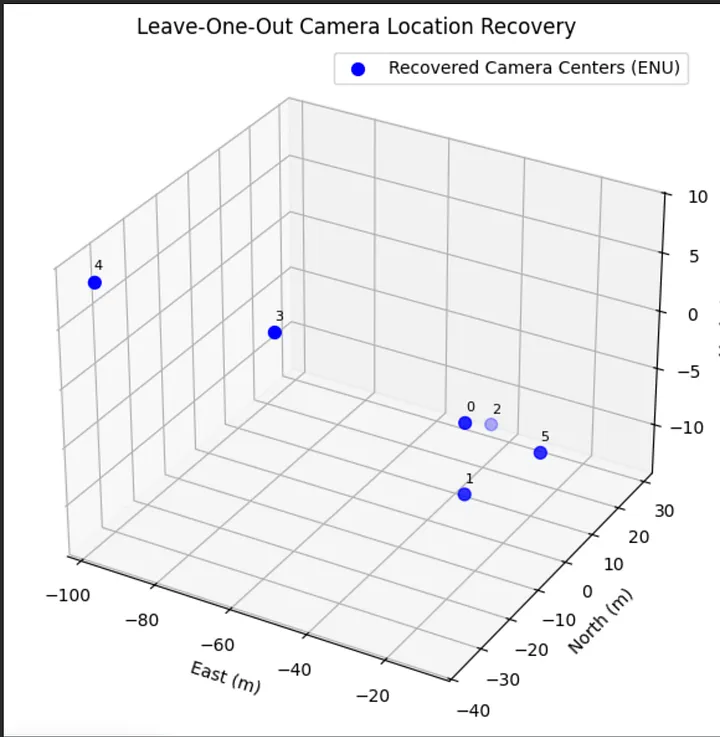
\includegraphics[width=0.7\textwidth]{figs/leave_one_out_camera_centers.png}
\caption{Centros da câmara recuperados (referencial ENU) nas execuções da análise \textit{leave-one-out}~\cite{sunkara2025}.}
\label{fig:sunkara_loo}
\end{figure}

Os resultados mostram que as estimativas são muito sensíveis a cada ponto individual. Com todos os pontos, o erro de reprojeção é de 39,40~px; ao retirar um ponto, varia entre 9,65~px (ponto 5) e 41,92~px (ponto 1). A distância focal estimada varia entre 1210,2 e 1933,8~px (HFOV entre $93{,}9^{\circ}$ e $67{,}7^{\circ}$), a componente vertical de $\mathbf{t}$ entre 11,00 e 98,27~m, e os centros da câmara recuperados dispersam-se por dezenas de metros (Figura~\ref{fig:sunkara_loo}). Como cada execução usa apenas cinco ou seis correspondências, o problema fica pouco condicionado. Uma redução do erro ao retirar um ponto (por exemplo, o ponto 5) pode indicar que esse ponto é inconsistente com os restantes, mas também resulta possivelmente por haver menos restrições a satisfazer, pelo que, por si só, não garante uma pose mais correta.

\paragraph{Parte 2: câmaras reais.} Valida o \textit{pipeline} com imagens de \textit{webcams} publicamente disponíveis de três locais da área de Boston. Para cada câmara, constrói um conjunto de dados de pontos de interesse (\textit{POI}) com as coordenadas de imagem e as coordenadas GPS de cada ponto, e repete a calibração com marcos conhecidos e posições GPS aproximadas~\cite{sunkara2025}. As Tabelas~\ref{tab:sunkara_reais_intr} e~\ref{tab:sunkara_reais_pose} resumem os resultados.

\begin{table}[htbp]
\centering
\caption{Distância focal, erro de reprojeção e campos de visão nos três locais reais (parte 2)~\cite{sunkara2025}. As dimensões da imagem foram deduzidas da posição do ponto principal.}
\label{tab:sunkara_reais_intr}
\small
\begin{tabular}{ccccccc}
\hline
\textbf{Local} & \textbf{Imagem (px)} & \textbf{$f$ inicial (px)} & \textbf{$f$ estimada (px)} & \textbf{Erro (px)} & \textbf{HFOV ($^{\circ}$)} & \textbf{VFOV ($^{\circ}$)} \\
\hline
1 & $2940\times1730$ & 1013,86 & 1021,30 & 18,11 & 110,42 & 80,53 \\
2 & $1920\times1080$ & 871,10 & 998,96 & 50,83 & 87,72 & 56,79 \\
3 & $1920\times1080$ & 2015,31 & 3236,62 & 5,61 & 46,62 & 26,71 \\
\hline
\end{tabular}
\end{table}

\begin{table}[htbp]
\centering
\caption{Pose estimada nos três locais reais, no referencial ENU (parte 2). O centro da câmara $\mathbf{C}$ do local~1 é o reportado pelo artigo~\cite{sunkara2025}; os dos locais 2 e 3 foram calculados a partir de $\mathbf{R}$ e $\mathbf{t}$ com a Equação~\eqref{eq:cam_center}.}
\label{tab:sunkara_reais_pose}
\small
\begin{tabular}{ccc}
\hline
\textbf{Local} & \textbf{$\mathbf{t}$ (m) [E, N, U]} & \textbf{$\mathbf{C}$ (m) [E, N, U]} \\
\hline
1 & [$-24{,}55$; $15{,}70$; $50{,}34$] & [$57{,}62$; $-0{,}33$; $7{,}94$] \\
2 & [$31{,}67$; $-35{,}04$; $23{,}08$] & [$5{,}87$; $-39{,}17$; $-34{,}56$] \\
3 & [$243{,}13$; $219{,}27$; $819{,}29$] & [$-588{,}39$; $521{,}17$; $400{,}76$] \\
\hline
\end{tabular}
\end{table}

Observa-se o seguinte:

\begin{itemize}
    \item O erro de reprojeção varia entre 5,61~px (local~3) e 50,83~px (local~2), sendo de 18,11~px no local~1.
    \item Em todos os locais, apenas a distância focal é efetivamente ajustada: o ponto principal e a igualdade $f_x=f_y$ mantêm-se, e os coeficientes de distorção são nulos. A variação da distância focal face à estimativa inicial é pequena no local~1 (cerca de 0,7\%), moderada no local~2 (cerca de 15\%) e grande no local~3 (cerca de 61\%).
    \item O local~3 tem o menor erro, o maior $f$ (3236,62~px) e o menor campo de visão (HFOV de $46{,}62^{\circ}$), com a câmara a cerca de 880~m da origem do referencial ENU, ao contrário dos locais 1 e 2, onde esta distância é de aproximadamente 58~m e 53~m.
    \item Para o local~2, o artigo apresenta também os valores de $Z$ no referencial da câmara dos pontos usados (entre cerca de 58 e 152~m), todos positivos, isto é, à frente da câmara.
    \item No local~1, o centro da câmara calculado com a Equação~\eqref{eq:cam_center} a partir de $\mathbf{R}$ e $\mathbf{t}$ coincide com o reportado pelo artigo.
\end{itemize}

O artigo conclui que o \textit{pipeline} combina calibração de câmara, análise de incerteza e validação com dados reais, e que é possível estimar os parâmetros intrínsecos e extrínsecos de uma câmara real usando apenas píxeis e coordenadas GPS, passando de um conjunto de dados controlado para \textit{webcams} reais~\cite{sunkara2025}.

\subsubsection{Limitações e Relação com os Restantes Trabalhos}

Os resultados dependem da qualidade das correspondências: o próprio artigo simula o erro de medição acrescentando ruído às coordenadas 2D e 3D, e usa posições GPS aproximadas na parte real~\cite{sunkara2025}, o que evidencia a sensibilidade do método à precisão da seleção manual de píxeis e das coordenadas GPS (um erro de alguns metros no ponto 3D tem um efeito maior quanto mais próximo estiver da câmara). A análise \textit{leave-one-out} (Tabela~\ref{tab:sunkara_loo}) confirma esta sensibilidade: retirar um único ponto de seis altera a distância focal estimada entre 1210 e 1934~px. O modelo não inclui coeficientes de distorção, pelo que a distorção das lentes, quando existe, não é modelada e pode contribuir para o erro de reprojeção, e os valores do campo de visão vertical usados na inicialização não são justificados. Trata-se, além disso, de uma câmara fixa e de uma calibração feita \textit{a posteriori} a partir de uma imagem, e não de uma calibração em tempo real num dispositivo móvel.
